\subsection{Design}
\paragraph{}
Für die Art der Benutzerinteraktion des Programms sind mehrere Ansätze denkbar.
Beispielsweise könnte das Programm mit jeweils verschiedenen Befehlen von der
Kommandozeile aus aufgerufen werden wie in Abb. \ref{simple-gui-example} dargestellt.
Alternativ könnte das Program, wie in Abb. \ref{graphical-gui-example} skizziert,
mit einer kompletten grafischen Oberfläche versehen werden.

\paragraph{}
Als pragmatischer, einfacher und funktionaler Ansatz wurde ein Mittelweg gewählt
bei dem eine einfache Konsolenanwendung beim Start alle einzelnen konfigurierten
Zielwerte auf jeweils einer Zeile darstellt, geöffnet bleibt und auf Tasteneingaben
wartet um entweder eine der Funktionen auszuführen oder beendet zu werden (siehe Abb. \ref{post-start}
im Kapitel \ref{Kundendokumentation} - Kundendokumentation).


\begin{figure}
    \caption{Nutzerinteraktion mit aufeinanderfolgenden Befehlen}
    \label{simple-gui-example}
    \begin{minted}[bgcolor=codebg]{bash}
        >_ terminal-config-manager show
    
        1 Anwendung a mit Wert -> b
        2 Anwendung c mit Wert -> d
    
        >_ terminal-config-manager change 2
    
        1 Anwendung a mit Wert -> b
        2 Anwendung c mit Wert -> e
    \end{minted}
\end{figure}

\begin{figure}
    \caption{Grafische Oberfläche, skizzenhaft}
    \label{graphical-gui-example}
    \centering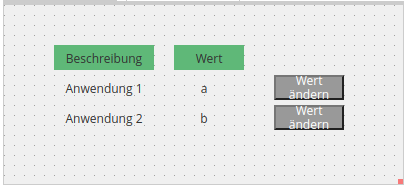
\includegraphics[scale=0.5]{gui-example.png}
\end{figure}
